\documentclass[12pt,a4paper]{article}

% ---------------- Packages ----------------
\usepackage[utf8]{inputenc}
\usepackage{geometry}
\usepackage{graphicx}
\usepackage{hyperref}
\usepackage{enumitem}
\usepackage{float}
\usepackage{titlesec}
\usepackage{fancyhdr}
\usepackage{tocloft}
\usepackage{xcolor}
\usepackage{tcolorbox}
\usepackage{parskip}

% ---------------- Color Scheme ----------------
\definecolor{primaryblue}{RGB}{0, 102, 204}
\definecolor{secondaryblue}{RGB}{51, 153, 255}
\definecolor{lightgray}{RGB}{245, 245, 245}

% ---------------- Formatting ----------------
\geometry{margin=1in, headheight=15pt}

% Section formatting
\titleformat{\section}
  {\Large\bfseries\color{primaryblue}}
  {\thesection}{1em}{}
  [\titlerule]

\titleformat{\subsection}
  {\large\bfseries\color{secondaryblue}}
  {\thesubsection}{1em}{}

\titleformat{\subsubsection}
  {\normalsize\bfseries}
  {\thesubsubsection}{1em}{}

% Header and Footer
\pagestyle{fancy}
\fancyhf{}
\fancyhead[L]{\small\textit{Food Truck Order Management System}}
\fancyhead[R]{\small\textit{SRS - Team Sleepers}}
\fancyfoot[C]{\thepage}
\renewcommand{\headrulewidth}{0.5pt}
\renewcommand{\footrulewidth}{0.5pt}

% Table of Contents formatting
\renewcommand{\cftsecleader}{\cftdotfill{\cftdotsep}}
\setlength{\cftbeforesecskip}{8pt}

% Hyperlink colors
\hypersetup{
    colorlinks=true,
    linkcolor=primaryblue,
    urlcolor=secondaryblue,
    citecolor=primaryblue
}

% Custom box for user stories
\newtcolorbox{storybox}{
    colback=lightgray,
    colframe=primaryblue,
    boxrule=0.5pt,
    arc=3pt,
    left=10pt,
    right=10pt,
    top=8pt,
    bottom=8pt
}

% ---------------- Document Info ----------------
\title{
    \vspace{2cm}
    {\Huge\bfseries\color{primaryblue} Software Requirements Specification} \\[1em]
    {\LARGE Food Truck Order Management System} \\[0.8em]
    \rule{\textwidth}{1.5pt} \\[0.8em]
    {\large\textit{Living Document – Agile Approach}} \\[2cm]
}

\author{
    {\Large\textbf{Team Sleepers}} \\[1.5em]
    \begin{tabular}{p{6cm}p{3cm}}
        Hassan Yousef & 13006567 \\ 
        Sara Adel & 14003723 \\
        Hana Yasser & 13003628 \\
        Mohamed Walid & 13006513 \\
        Omar Hani & 13007515 \\
        Abdelhamid ElSharnouby & 13006294 \\
        Hanin Mohamed & 13007010 \\
        Khaled Khaled & 14001048 \\
    \end{tabular} \\[2.5em]
    {\large\textbf{German International University (GIU)}} \\[2.5em]
    {\large\textbf{Supervised by:}} \\[0.8em]
    Dr.~Iman Awaad \\ 
    Eng.~Amir Haytham
}

\date{\large\today}

\begin{document}

% ---------------- Title Page ----------------
\maketitle
\thispagestyle{empty}
\newpage

% ---------------- Table of Contents ----------------
\tableofcontents
\thispagestyle{empty}
\newpage

% Reset page numbering
\setcounter{page}{1}

% ---------------- Section 1: Introduction ----------------
\section{Introduction}

\subsection{Purpose}

\begin{tcolorbox}[colback=primaryblue!5, colframe=primaryblue, boxrule=1pt, arc=4pt, left=12pt, right=12pt, top=10pt, bottom=10pt]
{\large\textbf{Problem Statement:}}

\vspace{0.3em}

Students and staff at GIU face significant challenges during peak hours when ordering food from campus food trucks. Long waiting lines, unclear preparation times, and lack of order visibility create frustration and time loss, especially between classes when time is limited.

\vspace{0.8em}

{\large\textbf{Solution:}}

\vspace{0.3em}

The GIU Food Truck Order Management System is a comprehensive web-based application designed to enable the members of the GIU community to reserve menu items from specific food trucks on campus for pick-up within a given time window, thus alleviating the problem with long waiting times for food and beverage items during peak periods in between classes. 

\vspace{0.5em}

This system enables seamless menu browsing, order placement, and order management for food truck customers as well as providing a similarly intuitive, efficient, and scalable solution for food service providers.
\end{tcolorbox}

\subsection{Intended Audience}
\begin{itemize}[leftmargin=2em, itemsep=8pt]
  \item \textbf{Project Team:} Hassan Yousef, Sara Adel, Hana Yasser, Mohamed Walid, Omar Hany, Abdelhamid ElSharnouby, Hanin Mohamed, Khaled Khaled.
  \item \textbf{Developers and Testers:} Project team members.
  \item \textbf{Product Owner:} Doctor Iman Awaad.
  \item \textbf{Instructors:} Dr.~Iman Awaad, Eng.~Amir Haytham and Eng.~Ahmad Sherif
\end{itemize}

\subsection{Scope}
The Food-truck System is a website that helps students and staff at GIU order food from the food trucks on campus. People can open the menus of different food trucks to see what food and drinks are available. They can then choose the items they want and make their order online. The system lets them pick up their food in a specific time, so they don't have to wait in long lines. This makes it easier for everyone to get their food, especially during busy times between classes. The system also helps the food trucks manage orders better, making sure everything runs smoothly for both customers and service providers. In general, the goal is to save time and make ordering food on campus simple and comfortable for the entire community.

\subsection{Overview}

\begin{tcolorbox}[colback=lightgray, colframe=secondaryblue, boxrule=0.8pt, arc=3pt, left=10pt, right=10pt, top=8pt, bottom=8pt]

The Food Truck Order Management System is a simple website for ordering food from the food trucks on the GIU campus. It helps to reduce waiting in lines by letting users place orders before going to the truck.

\vspace{0.5em}

{\bfseries\color{secondaryblue} Who uses it:}
\begin{itemize}[leftmargin=1.8em,itemsep=5pt, topsep=6pt]
  \item \textbf{Students and Staff (Customers):} Browse trucks, view menus, select items, place an order, choose (or accept) a pickup time, and check the order status (received, preparing, ready) on the website.
  \item \textbf{Food Truck Staff:} See incoming orders, update each order's status, manage menu items (add or remove).
  \item \textbf{Administrator:} Add or remove food trucks and oversee basic platform usage.
\end{itemize}

\vspace{0.3em}

{\bfseries\color{secondaryblue} How order tracking works:} The page refreshes (or auto-checks) every short interval to show updated order status. It does not use push notifications or advanced real-time technology.

\vspace{0.3em}

{\bfseries\color{secondaryblue} What it does NOT include:} No delivery, no online payment, no mobile app, no live chat, no push notifications, no multi-language (English only), no external integrations.

\vspace{0.3em}

{\bfseries\color{secondaryblue} Why provider hours are longer:} Food truck staff have extra time (before and after customer hours) to prepare ingredients and clean up.

\vspace{0.3em}

{\bfseries\color{secondaryblue} Main goal:} Save time, make ordering clearer and easier, and help trucks manage orders better.

\vspace{0.3em}

{\bfseries\color{secondaryblue} Other notes:} Works in a normal web browser on phones, tablets, and laptops. Designed for up to about 500 users at once.

\end{tcolorbox}

\newpage

% ---------------- Section 2: Product Vision & Scope ----------------
\section{Product Vision and Scope}

\subsection{Product Vision}

The \textbf{Food Truck Order Management System} envisions a seamless, digital-first campus dining experience that minimizes waiting time and optimizes operations for both customers and vendors. The system will serve as a centralized web platform connecting GIU students, staff, and food truck operators through a polling-based ordering process.

From a user perspective, the vision is to eliminate the inefficiency of physical queues by allowing users to browse menus, place customized orders, and schedule pickups in advance. For food truck operators, the platform provides a unified dashboard to manage incoming orders and track preparation progress. Administrators will be able to manage participating vendors, monitor overall platform activity, and ensure service quality across all trucks.

The long-term vision is to transform how on-campus food services operate — creating a scalable digital ecosystem that supports automated order tracking, predictive demand analytics, and an integrated payment experience. Ultimately, this system aims to enhance convenience, transparency, and satisfaction for the GIU community while providing actionable insights to vendors and administrators for continuous operational improvement.

\subsection{In Scope}
The system includes the following features as part of its core functionality, categorized by user role.

\subsubsection{Customer Features}
\begin{itemize}[leftmargin=2em, itemsep=6pt]
    \item \textbf{User Authentication:} Customers can register and log in using email and password.
    \item \textbf{Menu Browsing:} Users can browse a list of food trucks, then view each truck's menu of food items.
    \item \textbf{Online Ordering:} Customers can place orders and select pickup times.
    \item \textbf{Estimated Preparation Time:} The system displays estimated time before confirming an order.
    \item \textbf{Order Status Tracking:} Customers can track order progress (Pending, In Progress, Ready).
    \item \textbf{Busy Mode on menu:} Customers can see if a vendor is currently too busy to accept new orders.
\end{itemize}

\subsubsection{Vendor Features}
\begin{itemize}[leftmargin=2em, itemsep=6pt]
    \item \textbf{View and Manage Orders:} Vendors can view incoming orders and update their statuses.
    \item \textbf{Menu Management:} Vendors can add or remove menu items.
    \item \textbf{Activate Busy Mode:} Vendors can temporarily stop accepting new orders.
\end{itemize}

\subsubsection{Admin Features}
\begin{itemize}[leftmargin=2em, itemsep=6pt]
    \item \textbf{Food truck management:} Admin can add or remove food trucks.
\end{itemize}

\subsection{Out of Scope}
The following features are explicitly excluded from the current system scope:

\begin{itemize}[leftmargin=2em, itemsep=6pt]
    \item \textbf{Restaurant Rating:} Users cannot rate or review food trucks or individual menu items. No feedback mechanism or star rating system is included in this release.
    \item \textbf{Bestsellers Menu:} The system does not track or display popular items, trending dishes, or "most ordered" recommendations. No sales analytics or item popularity features are provided.
    \item \textbf{Mobile Application:} The system will only be accessible via web browsers; no Android or iOS apps are included in this release.
    \item \textbf{Online Payment Integration:} Users will not be able to pay online. All transactions will be handled offline or through existing university methods.
    \item \textbf{Delivery Services:} Food delivery is not supported. Customers must pick up their orders from the food trucks in person.
    \item \textbf{University Authentication System Integration:} The system does not connect to GIU's single sign-on or internal authentication infrastructure.
    \item \textbf{Push Notifications:} Real-time push notifications (e.g., mobile or browser alerts) are not supported in this release. Users must track their orders through the website interface.
    \item \textbf{Multiple Language Support:} The system will only support English in its initial release. Support for other languages is excluded from scope.
    \item \textbf{Live Chat or Messaging:} No communication feature (e.g., chat with vendors or support) is included.
    \item \textbf{Advanced Real-Time Communication:} The system will use simple periodic refresh or polling to check order updates. Advanced real-time communication technologies (WebSockets, Server-Sent Events) are not included in this version.
    \item \textbf{Third-Party Integrations:} No integration with external services (e.g., social media, third-party APIs) is planned.
    \item \textbf{Advanced Analytics:} The system will not include complex analytics or reporting features for vendors or administrators.
\end{itemize}

\newpage

% ---------------- Section 3: High-Level Architecture ----------------
\section{High-Level Architecture}

\begin{tcolorbox}[colback=primaryblue!5, colframe=primaryblue, boxrule=1pt, arc=3pt, left=10pt, right=10pt, top=8pt, bottom=8pt]
\begin{itemize}[leftmargin=2em, itemsep=10pt]
    \item \textbf{Front End:} Modern HTML, CSS, JavaScript, and jQuery. Or JavaScript Framework  
    \item \textbf{Back End:} RESTful API using Node.js
    \item \textbf{Database:} Relational (PostgreSQL)
    \item \textbf{Authentication:} Email/password authentication (no external OAuth)
    \item \textbf{Payment:} Currently, none (offline transactions only)
    \item \textbf{Hosting:} To be determined (university servers or cloud provider)
\end{itemize}
\end{tcolorbox}

\subsection{Password Security: Bcrypt Hashing Implementation}

\begin{tcolorbox}[colback=primaryblue!5, colframe=primaryblue, boxrule=1pt, arc=3pt, left=10pt, right=10pt, top=8pt, bottom=8pt]

\subsubsection{Purpose and Security Rationale}

The Food Truck Order Management System implements \textbf{bcrypt} as the cryptographic hashing algorithm for all user password storage. This industry-standard approach ensures that user credentials remain secure even in the event of database compromise, protecting students, staff, and vendors from unauthorized access.

\vspace{0.5em}

\textbf{Core Security Principles:}

\begin{itemize}[leftmargin=2em, itemsep=6pt]
    \item \textbf{Irreversibility:} Bcrypt is a one-way cryptographic function. Passwords cannot be reverse-engineered from stored hashes, ensuring that even system administrators cannot view user passwords.
    \item \textbf{Defense Against Rainbow Tables:} Built-in salt generation prevents attackers from using precomputed hash tables to crack passwords efficiently.
    \item \textbf{Computational Cost:} Bcrypt's adaptive work factor makes brute-force attacks computationally expensive and time-prohibitive.
    \item \textbf{Future-Proof Security:} The configurable cost factor allows increasing computational complexity as hardware capabilities improve.
\end{itemize}

\subsubsection{Why Bcrypt Over Alternative Approaches}

\textbf{Comparison with Other Hashing Methods:}

\begin{description}[leftmargin=2em, itemsep=8pt, style=nextline]
    \item[\textbf{MD5 and SHA-1 (Rejected):}] These algorithms are cryptographically broken and vulnerable to collision attacks. They hash passwords too quickly, enabling millions of guesses per second with modern GPUs.
    
    \item[\textbf{Plain SHA-256/SHA-512 (Insufficient):}] While cryptographically secure for integrity checking, these algorithms are too fast for password hashing. Without proper salting and key stretching, they remain vulnerable to brute-force attacks.
    
    \item[\textbf{PBKDF2 (Alternative):}] A viable alternative that provides key stretching, but bcrypt is specifically designed for password hashing with built-in salt management and has stronger resistance to GPU-based attacks.
    
    \item[\textbf{Argon2 (Future Consideration):}] The winner of the Password Hashing Competition (2015), Argon2 offers superior protection against GPU and ASIC attacks. However, bcrypt remains the industry standard with broader ecosystem support and proven security track record for web applications.
    
    \item[\textbf{Scrypt (Alternative):}] Provides memory-hard properties that resist hardware-based attacks, but bcrypt's maturity and widespread library support make it the preferred choice for this project's scope.
\end{description}

\vspace{0.5em}

\textbf{Decision Rationale:} Bcrypt strikes the optimal balance between proven security, performance, ecosystem maturity, and ease of implementation for a university-scale web application.

\subsubsection{Technical Implementation}

\textbf{Algorithm Mechanics:}

Bcrypt operates on the Blowfish cipher with an adaptive cost factor:

\begin{enumerate}[leftmargin=2em, itemsep=6pt]
    \item \textbf{Salt Generation:} A cryptographically random 128-bit salt is generated for each password.
    \item \textbf{Key Derivation:} The password and salt undergo multiple rounds of the Blowfish key schedule.
    \item \textbf{Work Factor Application:} The algorithm applies $2^{cost}$ iterations, where cost is configurable (typically 10-12).
    \item \textbf{Hash Output:} Produces a 60-character string containing the algorithm identifier, cost factor, salt, and hash.
\end{enumerate}

\vspace{0.5em}

\textbf{Hash Format Structure:}

\begin{verbatim}
$2b$12$R9h/cIPz0gi.URNNX3kh2OPST9/PgBkqquzi.Ss7KIUgO2t0jWMUW
|  |  |                     |
|  |  |                     |- 31-char hash
|  |  |- 22-char salt
|  |- Cost factor (2^12 = 4096 rounds)
|- Algorithm identifier (2b = bcrypt)
\end{verbatim}

\vspace{0.5em}

\textbf{Node.js Integration:}

The system utilizes the \texttt{bcrypt} npm package for implementation:

\begin{verbatim}
const bcrypt = require('bcrypt');
const SALT_ROUNDS = 12;

// Password hashing during registration
async function hashPassword(plainPassword) {
    const hashedPassword = await bcrypt.hash(
        plainPassword, 
        SALT_ROUNDS
    );
    return hashedPassword;
}

// Password verification during login
async function verifyPassword(plainPassword, hashedPassword) {
    const isValid = await bcrypt.compare(
        plainPassword, 
        hashedPassword
    );
    return isValid;
}
\end{verbatim}

\subsubsection{Security Configuration}

\textbf{Cost Factor Selection:}

The system employs a cost factor of \textbf{12}, resulting in $2^{12} = 4096$ hashing rounds. This configuration balances security and user experience:

\begin{itemize}[leftmargin=2em, itemsep=6pt]
    \item \textbf{Security Threshold:} At cost factor 12, hashing takes approximately 250-350ms on modern server hardware, making brute-force attacks impractical while remaining imperceptible to users during authentication.
    \item \textbf{Attack Resistance:} With 4096 rounds, an attacker attempting to crack a strong 10-character password would require centuries using standard computing resources.
    \item \textbf{Scalability Consideration:} Higher cost factors (13-14) may be implemented in future releases as hardware capabilities increase.
\end{itemize}

\vspace{0.5em}

\textbf{Salt Management:}

\begin{itemize}[leftmargin=2em, itemsep=6pt]
    \item Each password receives a unique, cryptographically random salt generated automatically by bcrypt.
    \item Salts are stored embedded within the hash output, eliminating separate salt storage requirements.
    \item Salt uniqueness ensures that identical passwords produce different hashes, preventing pattern detection.
\end{itemize}

\subsubsection{Integration Points}

\textbf{User Registration Flow:}

\begin{enumerate}[leftmargin=2em, itemsep=6pt]
    \item User submits registration form with email and password via HTTPS.
    \item Backend validates password strength requirements (minimum 8 characters, complexity rules).
    \item System hashes password using bcrypt with cost factor 12.
    \item Hashed password stored in PostgreSQL database; plaintext password never persisted.
    \item Registration confirmation sent to user without password exposure.
\end{enumerate}

\vspace{0.5em}

\textbf{Authentication Flow:}

\begin{enumerate}[leftmargin=2em, itemsep=6pt]
    \item User submits login credentials via HTTPS-secured connection.
    \item Backend retrieves stored hash from database based on email identifier.
    \item System uses bcrypt.compare() to verify submitted password against stored hash.
    \item On successful verification, JWT token or session cookie issued for authenticated access.
    \item Failed attempts logged for security monitoring and brute-force detection.
\end{enumerate}

\vspace{0.5em}

\textbf{Password Change Operations:}

\begin{enumerate}[leftmargin=2em, itemsep=6pt]
    \item User authenticates with current password using standard login verification.
    \item New password validated against strength requirements.
    \item New password hashed with fresh salt using bcrypt.
    \item Database updated with new hash; old hash overwritten and irrecoverable.
    \item Session invalidated, requiring re-authentication with new credentials.
\end{enumerate}

\subsubsection{Security Benefits and Threat Mitigation}

\textbf{Protection Against Common Attacks:}

\begin{description}[leftmargin=2em, itemsep=8pt, style=nextline]
    \item[\textbf{Database Breach:}] If the database is compromised, attackers obtain only bcrypt hashes. Without the original passwords, they cannot authenticate as legitimate users. Cracking individual hashes requires substantial computational resources.
    
    \item[\textbf{Brute-Force Attacks:}] The computational cost of bcrypt (approximately 250ms per attempt) limits attackers to roughly 4 password attempts per second per hash, making systematic brute-force attacks infeasible.
    
    \item[\textbf{Rainbow Table Attacks:}] Unique per-password salts render precomputed rainbow tables useless. Attackers must compute hashes individually for each password.
    
    \item[\textbf{Credential Stuffing:}] Even if users reuse passwords across platforms, bcrypt hashing ensures that compromised credentials from other breaches cannot be directly applied to this system.
    
    \item[\textbf{Insider Threats:}] System administrators and developers with database access cannot view user passwords, limiting insider risk and supporting principle of least privilege.
\end{description}

\subsubsection{Performance Considerations}

\textbf{System Impact:}

\begin{itemize}[leftmargin=2em, itemsep=6pt]
    \item \textbf{Registration Latency:} Password hashing adds approximately 250-350ms to registration time, imperceptible in typical user workflows.
    \item \textbf{Login Latency:} Authentication incurs similar 250-350ms overhead, acceptable for interactive login experiences.
    \item \textbf{Server Load:} Bcrypt is CPU-intensive but asynchronous implementation prevents blocking. Under peak load (500 concurrent users), authentication overhead remains manageable on modern multi-core servers.
    \item \textbf{Horizontal Scaling:} Bcrypt's CPU-bound nature scales horizontally with additional application server instances.
\end{itemize}

\vspace{0.5em}

\textbf{Rate Limiting Integration:}

To complement bcrypt's computational defenses, the system implements API-level rate limiting:

\begin{itemize}[leftmargin=2em, itemsep=6pt]
    \item Maximum 5 failed login attempts per email address within 15-minute window.
    \item Temporary account lockout (15 minutes) after threshold exceeded.
    \item Progressive delay increases with repeated failures.
    \item IP-based rate limiting prevents distributed brute-force attacks.
\end{itemize}

\subsubsection{Compliance and Best Practices}

\textbf{Industry Standards Alignment:}

\begin{itemize}[leftmargin=2em, itemsep=6pt]
    \item \textbf{OWASP Recommendations:} Bcrypt is explicitly recommended by OWASP (Open Web Application Security Project) for password storage.
    \item \textbf{NIST Guidelines:} Complies with NIST Special Publication 800-63B guidance on credential security.
    \item \textbf{GDPR Considerations:} Strong password hashing supports data protection requirements under privacy regulations.
\end{itemize}

\vspace{0.5em}

\textbf{Security Monitoring:}

The system implements logging and monitoring around bcrypt operations:

\begin{itemize}[leftmargin=2em, itemsep=6pt]
    \item Failed authentication attempts logged with timestamps and IP addresses.
    \item Anomalous patterns (rapid failed attempts, unusual access times) trigger security alerts.
    \item Password change operations audited for security review.
    \item Hash timing monitored to detect potential timing attack attempts.
\end{itemize}

\subsubsection{Future Enhancements}

\textbf{Planned Security Improvements:}

\begin{itemize}[leftmargin=2em, itemsep=6pt]
    \item \textbf{Adaptive Cost Factor:} Implement periodic cost factor increases as computing power advances (e.g., increment to 13 after two years).
    \item \textbf{Multi-Factor Authentication (MFA):} Add TOTP-based two-factor authentication to supplement password security.
    \item \textbf{Password Breach Detection:} Integrate with HaveIBeenPwned API to warn users of compromised passwords.
    \item \textbf{Migration to Argon2:} Evaluate migration to Argon2id for enhanced GPU resistance in future major releases.
\end{itemize}

\end{tcolorbox}

\subsection{Data Preservation Strategy: Soft Deletes}

\begin{tcolorbox}[colback=primaryblue!5, colframe=primaryblue, boxrule=1pt, arc=3pt, left=10pt, right=10pt, top=8pt, bottom=8pt]

\subsubsection{Purpose and Rationale}

The Food Truck Order Management System implements a \textbf{soft delete} mechanism as a core data preservation strategy to ensure business continuity, regulatory compliance, and operational integrity. Rather than permanently removing records from the database, soft deletes mark data as deleted while maintaining its physical presence in the system.

\vspace{0.5em}

\textbf{Key Objectives:}
\begin{itemize}[leftmargin=2em, itemsep=6pt]
    \item \textbf{Data Recovery:} Enable restoration of accidentally deleted records without requiring database backups.
    \item \textbf{Audit Trail:} Maintain complete historical records for compliance, reporting, and analysis purposes.
    \item \textbf{Referential Integrity:} Preserve relationships between orders, menu items, and users even after logical deletion.
    \item \textbf{Business Intelligence:} Retain historical data for trend analysis, seasonal patterns, and vendor performance metrics.
    \item \textbf{Legal Compliance:} Support potential retention policies and dispute resolution requirements.
\end{itemize}

\subsubsection{Implementation Architecture}

\textbf{Database Schema Design:}

Soft deletes are implemented through the addition of metadata columns to relevant database tables:

\begin{itemize}[leftmargin=2em, itemsep=8pt]
    \item \textbf{deleted\_at (TIMESTAMP):} Records the exact date and time when a record was logically deleted. NULL indicates an active record.
    \item \textbf{deleted\_by (INTEGER/VARCHAR):} Foreign key or identifier referencing the user who performed the deletion (admin, vendor, or system).
    \item \textbf{is\_deleted (BOOLEAN):} Optional flag for faster query indexing, typically derived from deleted\_at IS NOT NULL.
\end{itemize}

\vspace{0.5em}

\textbf{Affected Entities:}

The soft delete mechanism applies to the following core system entities:

\begin{itemize}[leftmargin=2em, itemsep=6pt]
    \item \textbf{Menu Items:} When vendors remove items from their menu, records remain in the database to preserve order history.
    \item \textbf{Food Trucks:} Deactivated or removed food trucks retain their data for historical order analysis and reporting.
    \item \textbf{User Accounts:} Deleted user accounts maintain order history and transaction records.
    \item \textbf{Orders:} While orders are rarely deleted, the system supports soft deletion for cancellations requiring audit trails.
\end{itemize}

\subsubsection{Application Layer Logic}

\textbf{Query Filtering:}

All standard application queries automatically exclude soft-deleted records through a consistent WHERE clause pattern:

\begin{verbatim}
SELECT * FROM menu_items 
WHERE deleted_at IS NULL;
\end{verbatim}

\vspace{0.5em}

\textbf{Deletion Operations:}

When a user or system process requests deletion, the application executes an UPDATE operation rather than DELETE:

\begin{verbatim}
UPDATE menu_items 
SET deleted_at = CURRENT_TIMESTAMP,
    deleted_by = current_user_id
WHERE item_id = target_id;
\end{verbatim}

\vspace{0.5em}

\textbf{Recovery Operations:}

Authorized administrators can restore soft-deleted records by setting deleted\_at to NULL:

\begin{verbatim}
UPDATE menu_items 
SET deleted_at = NULL,
    deleted_by = NULL
WHERE item_id = target_id;
\end{verbatim}

\subsubsection{System Impact and Considerations}

\textbf{Performance Implications:}

\begin{itemize}[leftmargin=2em, itemsep=6pt]
    \item \textbf{Storage Growth:} Database size increases over time as deleted records accumulate. Mitigation: Implement archival processes for records older than defined retention periods (e.g., 2 years).
    \item \textbf{Query Performance:} Additional WHERE clause filtering may impact query speed on large datasets. Mitigation: Create database indexes on deleted\_at columns.
    \item \textbf{Table Bloat:} PostgreSQL may experience table bloat with frequent soft deletes. Mitigation: Schedule periodic VACUUM operations.
\end{itemize}

\vspace{0.5em}

\textbf{Security and Access Control:}

\begin{itemize}[leftmargin=2em, itemsep=6pt]
    \item Soft-deleted records remain in the database and must be protected with appropriate access controls.
    \item Administrative interfaces for viewing deleted records require elevated permissions.
    \item Sensitive data in soft-deleted records (e.g., customer contact information) may require additional encryption or masking.
\end{itemize}

\vspace{0.5em}

\textbf{Referential Integrity:}

Soft deletes prevent foreign key constraint violations when related records exist:

\begin{itemize}[leftmargin=2em, itemsep=6pt]
    \item A menu item with existing orders cannot be hard deleted without cascading deletions or breaking order history.
    \item Soft deletion preserves the relationship, allowing historical orders to display accurate item details even after menu changes.
\end{itemize}

\subsubsection{User Experience Impact}

\textbf{For Customers:}
\begin{itemize}[leftmargin=2em, itemsep=6pt]
    \item Order history remains accessible even if menu items or food trucks are removed from active service.
    \item Past orders display correct item names and prices, maintaining transaction transparency.
\end{itemize}

\vspace{0.5em}

\textbf{For Vendors:}
\begin{itemize}[leftmargin=2em, itemsep=6pt]
    \item Removed menu items can be restored without re-entering all details if they return seasonally.
    \item Historical sales data remains available for business analytics and menu optimization.
\end{itemize}

\vspace{0.5em}

\textbf{For Administrators:}
\begin{itemize}[leftmargin=2em, itemsep=6pt]
    \item Complete platform activity history enables comprehensive reporting and dispute resolution.
    \item Accidentally removed food trucks can be restored without data loss.
\end{itemize}

\subsubsection{Data Lifecycle Management}

\textbf{Archival Policy:}

To balance data preservation with system performance, the following lifecycle management strategy is implemented:

\begin{enumerate}[leftmargin=2em, itemsep=6pt]
    \item \textbf{Active Retention (0-12 months):} All soft-deleted records remain in primary database tables, fully queryable through administrative interfaces.
    \item \textbf{Archive Phase (12-24 months):} Records may be migrated to separate archive tables or cold storage, reducing load on production queries.
    \item \textbf{Permanent Deletion (24+ months):} After the retention period expires, records may be permanently deleted following administrative approval and compliance verification.
\end{enumerate}

\vspace{0.5em}

\textbf{Compliance Considerations:}

The soft delete implementation supports compliance with potential data retention regulations:

\begin{itemize}[leftmargin=2em, itemsep=6pt]
    \item Transaction records for financial reconciliation and auditing purposes.
    \item User activity logs for security investigations and dispute resolution.
    \item Historical menu and pricing data for contract verification and vendor agreements.
\end{itemize}

\end{tcolorbox}

\newpage

% ---------------- Section 4: Functional Requirements ----------------
\section{Functional Requirements}

\subsection{User Stories}

\subsubsection{Food Truck Customer User Stories}
\begin{storybox}
\begin{itemize}[leftmargin=1em, itemsep=6pt]
    \item As a customer, I want to schedule my lunch order in advance so that I can check the order status through the website and know when my order is ready for pickup.
    \item As a customer, I want to browse all the food trucks available on campus, see all options.
\end{itemize}
\end{storybox}

\vspace{1em}

\subsubsection{Food Truck Service Provider User Stories}
\begin{storybox}
\begin{itemize}[leftmargin=1em, itemsep=6pt]
    \item As a food truck staff member, I want to receive new orders through the system and update order status (received, preparing, ready) so customers can track their orders via polling.
    \item As a food truck owner, I want to create my menu with items, prices, and cooking times.
\end{itemize}
\end{storybox}

\vspace{1em}

\subsubsection{Food Truck Admin User Stories}
\begin{storybox}
\begin{itemize}[leftmargin=1em, itemsep=6pt]
    \item As an administrator, I add or remove food trucks.
\end{itemize}
\end{storybox}

\subsection{Use Case Diagrams}

\begin{figure}[H]
    \centering
    \fbox{
\includegraphics[height=14cm]{cuc.png}}
    \caption{\textbf{Client Use Case Diagram}}
    \label{fig:client-usecase}
\end{figure}

\begin{figure}[H]
    \centering
    \fbox{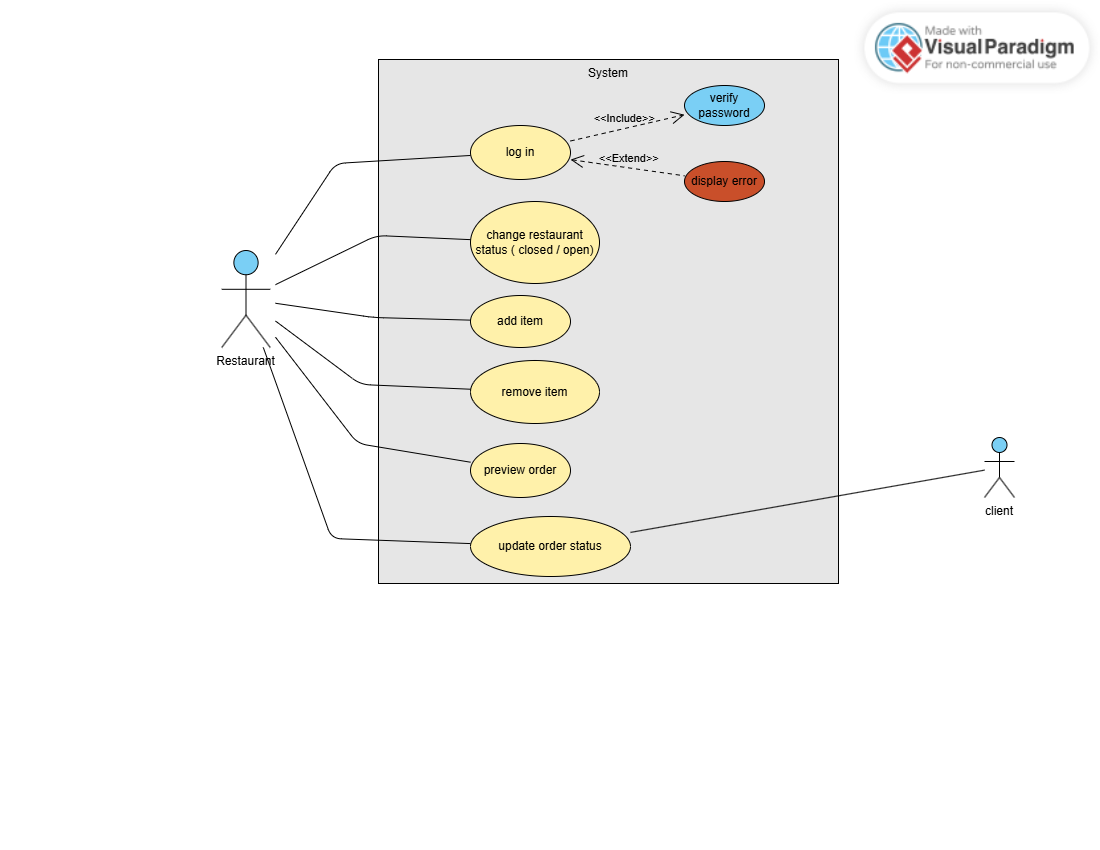
\includegraphics[height=14cm]{ruc.png}}
    \caption{\textbf{Restaurant Use Case Diagram}}
    \label{fig:restaurant-usecase}
\end{figure}

\begin{figure}[H]
    \centering
    \fbox{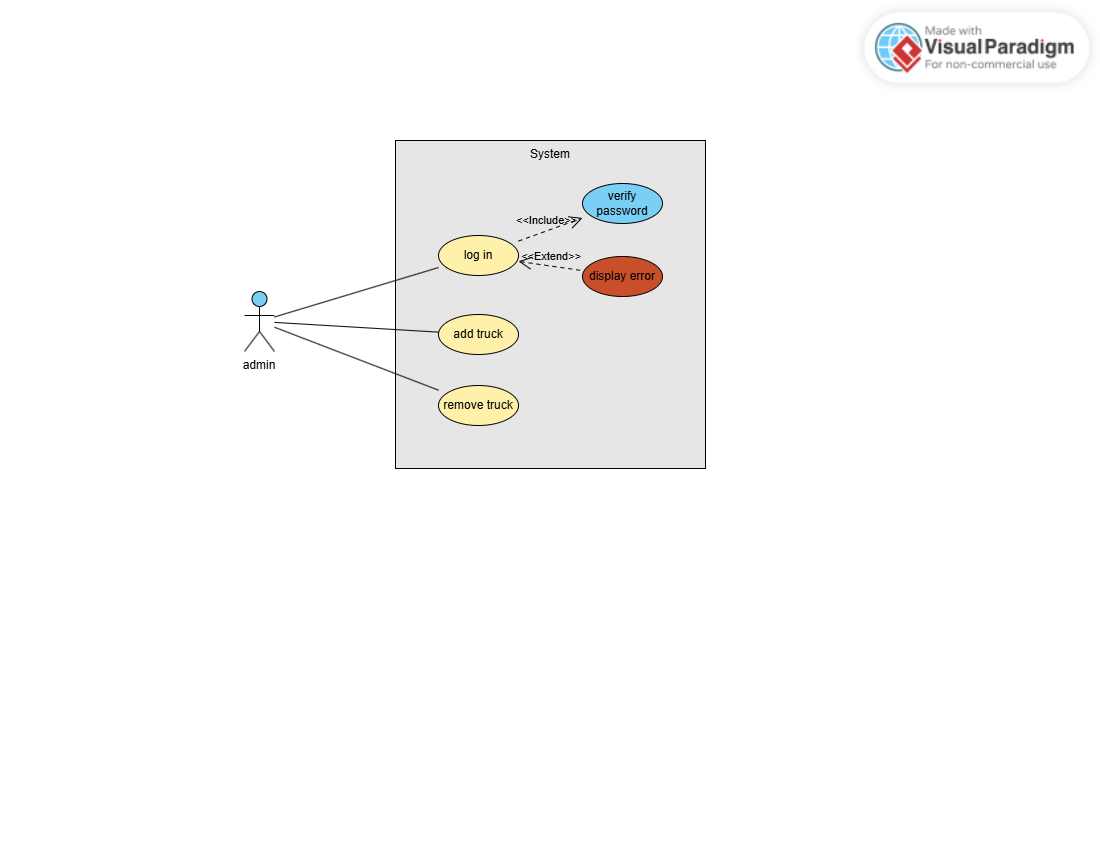
\includegraphics[height=14cm]{auc.png}}
    \caption{\textbf{Admin Use Case Diagram}}
    \label{fig:admin-usecase}
\end{figure}

\newpage

% ---------------- Section 5: Non-Functional Requirements ----------------
\section{Non-Functional Requirements}

\begin{tcolorbox}[colback=lightgray, colframe=primaryblue, boxrule=0.8pt, arc=3pt, left=10pt, right=10pt, top=8pt, bottom=8pt]
\begin{description}[leftmargin=2em, itemsep=12pt, style=nextline]
    \item[\textbf{Response Time:}] Page load times under three seconds.
    \item[\textbf{Concurrent Users:}] Support for at least 500 simultaneous users.
    \item[\textbf{API Security:}] Rate limiting and input validation.
    \item[\textbf{Backup \& Recovery:}] Automated daily backups with disaster recovery plan.
    \item[\textbf{System Operating Hours (Food Service Providers):}] 7:00 AM - 5:00 PM, Saturday to Thursday. This allows providers to prepare before customer ordering begins and complete cleanup after customer hours end.
    \item[\textbf{System Operating Hours (Food-truck Patrons):}] 8:00 AM - 4:40 PM, Saturday to Thursday.
\end{description}
\end{tcolorbox}

\newpage

% ---------------- Section 6: Interface Requirements ----------------
\section{Interface Requirements}
Currently, no external integrations (e.g. credit card, external authentication).

\newpage

% ---------------- Section 7: Constraints ----------------
\section{Constraints}

\subsection{Technical Constraints}
\begin{itemize}[leftmargin=2em, itemsep=8pt]
    \item \textbf{Web-Based Platform:} The system must be accessible via standard web browsers (Chrome, Firefox, Safari, Edge) without requiring native mobile applications in the initial release.
    \item \textbf{Technology Stack:} Development is limited to technologies and frameworks approved by GIU's IT infrastructure and familiar to the development team.
    \item \textbf{Database Management:} Must utilize a relational database system compatible with university hosting environments.
    \item \textbf{No External Payment Integration:} The initial version will not integrate third-party payment gateways; transactions will be handled offline or through existing university payment systems.
    \item \textbf{Campus Network Dependency:} Optimal performance is guaranteed only within GIU campus network infrastructure.
\end{itemize}

\subsection{Operational Constraints}
\begin{itemize}[leftmargin=2em, itemsep=8pt]
    \item \textbf{Operating Hours:} System functionality is limited to food truck operational hours (7:00 AM - 5:00 PM for providers, 8:00 AM - 4:40 PM for customers, Saturday to Thursday). The extended provider hours allow for preparation before service and cleanup after service.
    \item \textbf{Physical Pickup Required:} Orders must be physically collected from food trucks; no delivery service is provided.
    \item \textbf{Campus-Only Service:} The system serves only GIU campus food trucks and is geographically restricted to on-campus operations.
    \item \textbf{Manual Order Fulfillment:} Food preparation and handoff processes remain manual; the system only manages digital ordering and tracking.
\end{itemize}

\subsection{Resource Constraints}
\begin{itemize}[leftmargin=2em, itemsep=8pt]
    \item \textbf{Development Timeline:} The project must be completed within the academic semester timeframe as defined by the course requirements.
    \item \textbf{Team Size:} Development is limited to an 8-member student team with varying levels of experience.
    \item \textbf{Budget Limitations:} No dedicated budget for premium third-party services, APIs, or cloud infrastructure beyond what GIU provides.
    \item \textbf{Hardware Infrastructure:} Dependent on existing GIU server infrastructure and food truck operator devices (smartphones, tablets, or PCs).
\end{itemize}

\subsection{Regulatory and Policy Constraints}
\begin{itemize}[leftmargin=2em, itemsep=8pt]
    \item \textbf{Data Privacy Compliance:} Must adhere to GIU's data protection policies and student information privacy guidelines.
    \item \textbf{University Authentication:} Initial version will not integrate with GIU's central authentication system (planned for future releases).
    \item \textbf{Food Safety Standards:} The system does not enforce or monitor food safety regulations; responsibility remains with food truck operators.
    \item \textbf{Vendor Agreements:} Participation of food trucks is subject to approval and agreements with GIU administration.
\end{itemize}

\subsection{User and Usability Constraints}
\begin{itemize}[leftmargin=2em, itemsep=8pt]
    \item \textbf{Internet Connectivity:} Users must have stable internet connection to access the system; no offline functionality is provided.
    \item \textbf{Device Requirements:} Users need devices with modern web browsers; minimum screen size recommendations apply for optimal experience.
    \item \textbf{Digital Literacy:} Assumes basic computer and smartphone literacy among students, staff, and food truck operators.
    \item \textbf{Language Support:} Initial release supports English only; Arabic language support planned for future versions.
\end{itemize}

\subsection{Design and Architectural Constraints}
\begin{itemize}[leftmargin=2em, itemsep=8pt]
    \item \textbf{Scalability Scope:} System designed for GIU campus scale (approximately 500 concurrent users); not architected for multi-campus deployment in initial version.
    \item \textbf{Polling-Based Updates:} Order status updates operate on polling or periodic refresh mechanisms, not true real-time WebSocket connections.
    \item \textbf{Legacy System Integration:} No integration with existing GIU administrative systems (student information, financial systems) in the initial release.
    \item \textbf{Responsive Design Mandatory:} Must function across desktop, tablet, and mobile screen sizes despite being web-only.
\end{itemize}

\newpage

% ---------------- Section 8: CI/CD Pipeline ----------------
\section{Continuous Integration and Continuous Deployment Pipeline}

\subsection{Overview and Purpose}

The Food Truck Order Management System implements a robust \textbf{CI/CD (Continuous Integration/Continuous Deployment)} pipeline to automate the software development lifecycle, ensuring rapid, reliable, and repeatable deployments. This automated workflow enables the development team to deliver features, bug fixes, and security updates with confidence while maintaining system stability and minimizing manual intervention.

\begin{tcolorbox}[colback=primaryblue!5, colframe=primaryblue, boxrule=1pt, arc=3pt, left=10pt, right=10pt, top=8pt, bottom=8pt]

\textbf{Key Objectives:}

\begin{itemize}[leftmargin=2em, itemsep=6pt]
    \item \textbf{Automated Testing:} Execute comprehensive test suites on every code change to catch bugs early in the development cycle.
    \item \textbf{Code Quality Assurance:} Enforce coding standards, security best practices, and maintainability through automated analysis.
    \item \textbf{Rapid Feedback:} Provide developers with immediate feedback on code quality and test results within minutes of pushing changes.
    \item \textbf{Deployment Automation:} Eliminate manual deployment steps, reducing human error and accelerating release cycles.
    \item \textbf{Environment Consistency:} Ensure identical deployment processes across development, staging, and production environments.
    \item \textbf{Rollback Capability:} Enable quick reversion to previous stable versions if issues are detected post-deployment.
\end{itemize}

\end{tcolorbox}

\subsection{Pipeline Architecture}

\subsubsection{Technology Stack}

\begin{description}[leftmargin=2em, itemsep=8pt, style=nextline]
    \item[\textbf{Version Control:}] Git with GitHub as the central repository hosting platform.
    
    \item[\textbf{CI/CD Platform:}] GitHub Actions for pipeline orchestration and automation workflows.
    
    \item[\textbf{Containerization:}] Docker for creating consistent, portable application environments across all deployment stages.
    
    \item[\textbf{Testing Frameworks:}] 
    \begin{itemize}[leftmargin=2em, itemsep=4pt]
        \item Jest for JavaScript unit and integration testing
        \item Supertest for API endpoint testing
        \item Playwright or Cypress for end-to-end browser testing
    \end{itemize}
    
    \item[\textbf{Code Quality Tools:}]
    \begin{itemize}[leftmargin=2em, itemsep=4pt]
        \item ESLint for JavaScript code linting and style enforcement
        \item Prettier for consistent code formatting
        \item SonarQube or CodeClimate for code quality metrics and technical debt analysis
    \end{itemize}
    
    \item[\textbf{Security Scanning:}]
    \begin{itemize}[leftmargin=2em, itemsep=4pt]
        \item npm audit for dependency vulnerability scanning
        \item Snyk or Dependabot for automated security patch suggestions
        \item OWASP Dependency-Check for known vulnerability detection
    \end{itemize}
\end{description}

\subsubsection{Pipeline Stages}

The CI/CD pipeline consists of sequential stages that must pass before code reaches production:

\begin{tcolorbox}[colback=lightgray, colframe=secondaryblue, boxrule=0.8pt, arc=3pt, left=10pt, right=10pt, top=8pt, bottom=8pt]

\textbf{Stage 1: Code Commit and Trigger}

\begin{itemize}[leftmargin=2em, itemsep=6pt]
    \item Developer commits code to feature branch and pushes to GitHub.
    \item GitHub webhook triggers CI/CD pipeline automatically.
    \item Pipeline executes on pull request creation, update, or merge to main branches.
\end{itemize}

\vspace{0.5em}

\textbf{Stage 2: Build and Environment Setup}

\begin{itemize}[leftmargin=2em, itemsep=6pt]
    \item Checkout source code from repository.
    \item Set up Node.js environment (v18 or v20 LTS).
    \item Install project dependencies using \texttt{npm ci} for reproducible builds.
    \item Compile TypeScript (if applicable) and bundle frontend assets.
    \item Build Docker images for backend and frontend services.
\end{itemize}

\vspace{0.5em}

\textbf{Stage 3: Static Code Analysis}

\begin{itemize}[leftmargin=2em, itemsep=6pt]
    \item Run ESLint to detect code quality issues, unused variables, and anti-patterns.
    \item Execute Prettier to verify code formatting consistency.
    \item Perform SonarQube analysis for code complexity, duplication, and maintainability metrics.
    \item Generate code coverage reports to ensure adequate test coverage (minimum 70\% threshold).
\end{itemize}

\vspace{0.5em}

\textbf{Stage 4: Automated Testing}

\begin{itemize}[leftmargin=2em, itemsep=6pt]
    \item \textbf{Unit Tests:} Execute isolated tests for individual functions and components (target: 80\% coverage).
    \item \textbf{Integration Tests:} Verify interactions between modules, database operations, and API endpoints.
    \item \textbf{API Tests:} Validate RESTful API contracts, response formats, and error handling.
    \item \textbf{End-to-End Tests:} Simulate complete user workflows in headless browser environments.
    \item All tests must pass with zero failures before proceeding.
\end{itemize}

\vspace{0.5em}

\textbf{Stage 5: Security Scanning}

\begin{itemize}[leftmargin=2em, itemsep=6pt]
    \item Run \texttt{npm audit} to identify vulnerable dependencies.
    \item Execute OWASP Dependency-Check for known CVE (Common Vulnerabilities and Exposures).
    \item Scan Docker images for security vulnerabilities using Trivy or Clair.
    \item Block deployment if critical or high-severity vulnerabilities detected.
\end{itemize}

\vspace{0.5em}

\textbf{Stage 6: Staging Deployment}

\begin{itemize}[leftmargin=2em, itemsep=6pt]
    \item Deploy application to staging environment (identical to production configuration).
    \item Execute smoke tests to verify critical functionality (login, order placement, status updates).
    \item Run performance tests to ensure response times meet non-functional requirements.
    \item Manual review and approval required before production deployment (for critical releases).
\end{itemize}

\vspace{0.5em}

\textbf{Stage 7: Production Deployment}

\begin{itemize}[leftmargin=2em, itemsep=6pt]
    \item Deploy Docker containers to production servers using rolling update strategy.
    \item Update database schema using migration scripts (with automatic rollback on failure).
    \item Execute health checks to confirm successful deployment.
    \item Monitor application logs and error rates during initial deployment period.
    \item Automatically rollback if error thresholds exceeded or health checks fail.
\end{itemize}

\vspace{0.5em}

\textbf{Stage 8: Post-Deployment Verification}

\begin{itemize}[leftmargin=2em, itemsep=6pt]
    \item Execute production smoke tests to verify core functionality.
    \item Monitor key performance indicators (response time, error rate, database connections).
    \item Send deployment notifications to team via Slack or email.
    \item Tag release in Git repository with version number and changelog.
\end{itemize}

\end{tcolorbox}

\subsection{Branching Strategy and Workflow}

\subsubsection{Git Branching Model}

The project employs a modified \textbf{Git Flow} branching strategy optimized for continuous deployment:

\begin{description}[leftmargin=2em, itemsep=8pt, style=nextline]
    \item[\textbf{main Branch:}] Production-ready code. All commits to main trigger automatic production deployment after passing all pipeline stages. Protected branch requiring pull request reviews.
    
    \item[\textbf{develop Branch:}] Integration branch for ongoing development. Merges from feature branches undergo full CI testing. Automatically deploys to staging environment.
    
    \item[\textbf{feature/* Branches:}] Individual feature development. Naming convention: \texttt{feature/description-of-feature}. Triggers CI pipeline on push and pull request. Deleted after merge to develop.
    
    \item[\textbf{bugfix/* Branches:}] Bug fixes during development cycle. Similar workflow to feature branches. Naming: \texttt{bugfix/issue-description}.
    
    \item[\textbf{hotfix/* Branches:}] Emergency production fixes. Branched directly from main, merged to both main and develop. Triggers expedited pipeline with production deployment.
    
    \item[\textbf{release/* Branches:}] Release preparation and stabilization. Branched from develop when features are complete. Undergo final testing before merging to main.
\end{description}

\subsubsection{Pull Request Workflow}

\begin{enumerate}[leftmargin=2em, itemsep=6pt]
    \item Developer creates feature branch from develop.
    \item Implements feature with regular commits and pushes to remote.
    \item Creates pull request targeting develop branch.
    \item Automated CI pipeline executes (build, test, lint, security scan).
    \item Code review required from at least one team member.
    \item All CI checks must pass (green status) before merge allowed.
    \item Conflicts resolved, pull request approved and merged.
    \item Feature branch automatically deleted, develop branch deploys to staging.
\end{enumerate}

\subsection{Environment Management}

\subsubsection{Environment Tiers}

\begin{description}[leftmargin=2em, itemsep=8pt, style=nextline]
    \item[\textbf{Development Environment:}] Local developer machines with Docker Compose for running full stack (Node.js backend, PostgreSQL database, frontend). Environment variables stored in \texttt{.env.development} (git-ignored).
    
    \item[\textbf{Staging Environment:}] Cloud-hosted environment mirroring production configuration. Automatically updated on develop branch merges. Uses separate PostgreSQL database with production-like data volume. Accessible only within GIU network or via VPN.
    
    \item[\textbf{Production Environment:}] Live system serving GIU campus users. Deployed only from main branch after manual approval. High availability configuration with load balancing. Strict access controls and monitoring.
\end{description}

\subsubsection{Configuration Management}

\begin{itemize}[leftmargin=2em, itemsep=6pt]
    \item Environment-specific variables (database credentials, API keys) stored in GitHub Secrets.
    \item Configuration injected at deployment time, never committed to repository.
    \item Separate secrets for staging and production environments.
    \item Secret rotation performed quarterly or immediately after team member departure.
\end{itemize}

\subsection{Automated Testing Strategy}

\subsubsection{Test Coverage Requirements}

\begin{tcolorbox}[colback=lightgray, colframe=primaryblue, boxrule=0.8pt, arc=3pt, left=10pt, right=10pt, top=8pt, bottom=8pt]

\begin{itemize}[leftmargin=2em, itemsep=8pt]
    \item \textbf{Overall Code Coverage:} Minimum 70\% line coverage across entire codebase.
    \item \textbf{Critical Path Coverage:} 100\% coverage for authentication, order processing, and payment-related code.
    \item \textbf{API Endpoint Coverage:} All RESTful endpoints must have corresponding integration tests.
    \item \textbf{Regression Test Suite:} Automated tests for all previously discovered bugs to prevent reoccurrence.
\end{itemize}

\end{tcolorbox}

\subsubsection{Test Types and Execution}

\begin{description}[leftmargin=2em, itemsep=8pt, style=nextline]
    \item[\textbf{Unit Tests:}] Test individual functions, components, and utility methods in isolation. Executed on every commit (fastest feedback, typically completes in under 30 seconds).
    
    \item[\textbf{Integration Tests:}] Verify interactions between modules, database queries, and external service calls. Use test database seeded with consistent fixtures. Execute on pull requests and develop/main merges.
    
    \item[\textbf{API Tests:}] Validate HTTP endpoints, request/response formats, status codes, and error handling. Test authentication flows, authorization rules, and rate limiting. Run on staging environment after deployment.
    
    \item[\textbf{End-to-End Tests:}] Simulate complete user workflows (registration, login, browse menu, place order, track status). Execute in headless browser against staging environment. Run nightly and before production deployments.
    
    \item[\textbf{Performance Tests:}] Load testing with simulated concurrent users (target: 500 simultaneous users). Stress testing to identify breaking points and resource constraints. Execute weekly on staging environment.
\end{description}

\subsection{Deployment Strategies}

\subsubsection{Rolling Deployment}

Production deployments use a \textbf{rolling update} strategy to minimize downtime:

\begin{enumerate}[leftmargin=2em, itemsep=6pt]
    \item New application version deployed to subset of servers (e.g., 25\% of instances).
    \item Health checks verify successful startup and functionality.
    \item If healthy, deployment continues to next batch of servers.
    \item Process repeats until all servers updated.
    \item Zero downtime achieved as old instances remain active until new ones ready.
    \item Automatic rollback if health checks fail at any stage.
\end{enumerate}

\subsubsection{Database Migration Handling}

\begin{itemize}[leftmargin=2em, itemsep=6pt]
    \item Schema changes managed through versioned migration scripts (using tool like Flyway or db-migrate).
    \item Migrations execute automatically before application deployment.
    \item Backward-compatible migrations ensure old application versions continue functioning during rolling updates.
    \item Database backups created automatically before migration execution.
    \item Migration failures trigger automatic rollback and deployment abortion.
\end{itemize}

\subsection{Monitoring and Observability}

\subsubsection{Pipeline Monitoring}

\begin{itemize}[leftmargin=2em, itemsep=6pt]
    \item GitHub Actions dashboard displays pipeline status, execution time, and failure patterns.
    \item Slack/email notifications sent on pipeline failures with error details and logs.
    \item Weekly pipeline metrics reported: success rate, average execution time, flaky test identification.
    \item Failed builds block merging and trigger immediate team notification.
\end{itemize}

\subsubsection{Application Monitoring Post-Deployment}

\begin{itemize}[leftmargin=2em, itemsep=6pt]
    \item Application performance monitoring (APM) tracks response times, error rates, and resource utilization.
    \item Log aggregation centralizes application logs from all servers for analysis and troubleshooting.
    \item Automated alerts triggered on error rate spikes, performance degradation, or service unavailability.
    \item Dashboards display key metrics: active users, order volume, API response times, database query performance.
\end{itemize}

\subsection{Security and Compliance}

\subsubsection{Pipeline Security}

\begin{itemize}[leftmargin=2em, itemsep=6pt]
    \item GitHub Actions workflows execute in isolated containers with minimal permissions.
    \item Secrets encrypted at rest and decrypted only during pipeline execution.
    \item Dependency updates automatically tested and reviewed before merging (Dependabot integration).
    \item Audit logs maintained for all deployments, including who approved and when.
\end{itemize}

\subsubsection{Access Controls}

\begin{itemize}[leftmargin=2em, itemsep=6pt]
    \item Production deployments require manual approval from designated team leads.
    \item GitHub branch protection rules enforce code review requirements and status checks.
    \item SSH keys and cloud credentials rotated regularly and stored securely.
    \item Principle of least privilege applied to all service accounts and deployment permissions.
\end{itemize}

\subsection{Benefits and Impact}

\begin{tcolorbox}[colback=primaryblue!10, colframe=primaryblue, boxrule=1pt, arc=4pt, left=10pt, right=10pt, top=8pt, bottom=8pt]

\textbf{Development Velocity:}

\begin{itemize}[leftmargin=2em, itemsep=6pt]
    \item Reduced deployment time from hours to minutes through automation.
    \item Faster feedback loops enable rapid iteration and bug fixing.
    \item Developers focus on coding rather than manual testing and deployment tasks.
\end{itemize}

\vspace{0.5em}

\textbf{Quality Assurance:}

\begin{itemize}[leftmargin=2em, itemsep=6pt]
    \item Automated testing catches bugs before they reach production.
    \item Consistent code quality through enforced linting and formatting standards.
    \item Security vulnerabilities identified and addressed early in development cycle.
\end{itemize}

\vspace{0.5em}

\textbf{Reliability and Stability:}

\begin{itemize}[leftmargin=2em, itemsep=6pt]
    \item Repeatable, automated deployments eliminate human error.
    \item Quick rollback capability minimizes impact of defects.
    \item Staging environment catches issues before production exposure.
\end{itemize}

\vspace{0.5em}

\textbf{Team Collaboration:}

\begin{itemize}[leftmargin=2em, itemsep=6pt]
    \item Transparent pipeline status visible to entire team.
    \item Code review process integrated into CI/CD workflow.
    \item Shared responsibility for code quality and deployment success.
\end{itemize}

\end{tcolorbox}

\newpage

% ---------------- Section 9: Future Scope ----------------
\section{Future Scope of the Project}
Potential features for future versions:
\begin{itemize}[leftmargin=2em, itemsep=8pt]
    \item Integration with university authentication.
    \item Push notifications for order updates.
    \item Mobile app version.
    \item Payment gateway support.
    \item \textbf{Rating and Review System:} Allow customers to rate food trucks and menu items, providing feedback and helping others make informed choices.
    \item \textbf{Inventory Management:} Enable vendors to track stock levels, receive low-stock alerts, and automatically mark items as unavailable when ingredients run out.
\end{itemize}

\newpage

% ---------------- Notes ----------------
\section*{Notes}
\addcontentsline{toc}{section}{Notes}

\begin{tcolorbox}[colback=yellow!10, colframe=orange!75!black, title=Important Note]
\begin{itemize}[leftmargin=1em]
    \item This is a \textbf{living document}. It evolves with project development.
    \item At the end, this document may be retitled as "Project Documentation."
\end{itemize}
\end{tcolorbox}

\vspace{1.5em}

\begin{tcolorbox}[colback=primaryblue!10, colframe=primaryblue, boxrule=1pt, arc=4pt, title=How the System Solves the Problem]

\textbf{The Challenge:} Students and staff waste valuable time standing in long queues at food trucks during peak hours, with no visibility into wait times or order status.

\vspace{0.5em}

\textbf{Our Solution:}

\begin{enumerate}[leftmargin=2em, itemsep=6pt]
    \item \textbf{Pre-ordering eliminates queues:} Users browse menus and place orders online before arriving at the truck, eliminating the need to wait in physical lines.
    
    \item \textbf{Time visibility reduces uncertainty:} The system displays estimated preparation times and allows users to select pickup windows, helping them plan their schedule.
    
    \item \textbf{Order tracking provides transparency:} Customers can check their order status (Pending → In Progress → Ready) through polling-based updates on the website, knowing exactly when to pick up their food.
    
    \item \textbf{Busy mode prevents overload:} Vendors can activate busy mode when overwhelmed, preventing new orders and managing capacity effectively.
    
    \item \textbf{Centralized platform streamlines operations:} Both customers and vendors access a single unified system, reducing confusion and improving coordination.
\end{enumerate}

\vspace{0.5em}

\textbf{Result:} Students and staff save time, avoid frustration, and enjoy a smoother campus dining experience, while food truck operators manage orders more efficiently and serve customers better.

\end{tcolorbox}

\end{document}